\documentclass[12pt, a4paper]{article}
\usepackage[utf8]{inputenc}
\usepackage{graphicx}

% Update this information to reflect yourself
\title{Assignment 1: Data Pipelines}
\author{Laurenz Aisenpreis}
\date{2021-09-29}

\begin{document}
\maketitle

\section{Introduction}

The following report discusses my implementation of a data pipeline to predict wind power production in Orkney. The data pipeline combines data from two different data sources, namely wind generation data and weather forecast data including the wind speed and direction.  
The application has been implemented by using the libraries \emph{sklearn} and \emph{pandas}.

\section{Pre-Pipeline Data Processing}

Some crucial preprocessing steps were performed before parsing the data into the pipeline. Most importantly, the timestamps of the two data sources had to be aligned. I took the decision, to query the wind generation data grouped by a period of three hours and summed up the total wind power generated within this time frame.
Following this, the two data sources were merged and the columns \emph{Lead hours} and \emph{Source time} were dropped. Those attributes were not taken into consideration, because the correlation matrix revealed a negative correlation between \emph{Source time} and \emph{Total}, and \emph{Lead hours} was simply a constant value. The main attributes for my analysis were therefore \emph{Speed} and \emph{Direction} to predict the \emph{Total} of generated wind. How those attributes were prepared is described in the next section.

\section{Data Pipeline}

In order to prepare the data set and conduct the prediction, both \emph{ColumnTransformer} and \emph{Pipeline} were used. Since the features of my model were a mix of numerical and categorical data, I decided to treat them differently. Within a \emph{ColumnTransformer}, first the missing values of the numerical feature \emph{Speed} were replaced by the median and scaled using the \emph{StandardScaler}. Secondly, the categorical feature \emph{Direction} was one hot encoded, to be able to interpret this attribute as a numerical value. \newline
Finally, my pipeline incorporated the transformations of the \emph{ColumnTransformer} and further transformed this data into polynomial combinations using \emph{PolynomialFeatures} to account for the non-linear nature of the input data. As the last step, I included the predictor of my choice and analyzed how the linear regression and k-nearest neighbor regressor models perform on the data set.

\section{Prediction Model Results and Evaluation}

The linear regression model achieved a score of \emph{0.73}. Especially the inclusion of polynomial transformation led to a relative increase of \emph{12.3} percent of accuracy compared to a previous score of \emph{0.65}. This can be explained by a better fit of the polynomially transformed model due to the non-linear relationship of the underlying data. \emph{Figure 1} depicts the regression line of the fitted model on the test data.

\begin{figure}[htp]
    \centering
    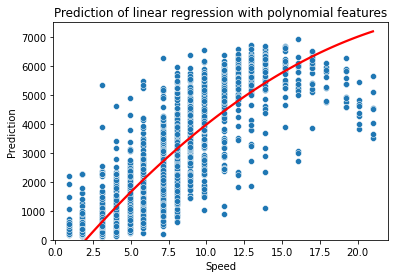
\includegraphics[width=12cm]{output_ln.png}
    \caption{Linear regression prediction}
    \label{fig:galaxy}
\end{figure}

The k-nearest neighbor model is another algorithm that can be used to approximate a dependent variable based on the \emph{neighborhood} of the independent variable values. However, k-NN with a neighbors-value set to 10 scored slightly worse than the linear regression model with a score of \emph{0.71}. The following \emph{Figure 2} shows the predictions of the k-NN model.

\begin{figure}[htp]
    \centering
    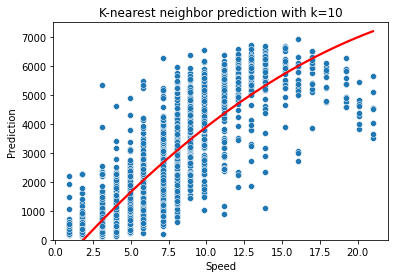
\includegraphics[width=12cm]{output_KNN.png}
    \caption{K-NN regression prediction}
    \label{fig:galaxy}
\end{figure}

As the last step, k-fold cross validation was applied to determine the accuracy of both models. A split size of 3 was used and resulted in an accuracy of \emph{0.71} for the \emph{linear regression} model and \emph{0.68} for the \emph{k-NN} model. Both with a standard deviation below \emph{0.01}.

\section{Conclusion}

These findings have shown that the linear regression model performed slightly better than the k-NN model, but could still not achieve a satisfying score.
Hence, the underlying data set must be improved to yield better results. My investigations have revealed that simply increasing the size of the data set does not necessarily improve the score of the model. A data set containing records of the past 2.000 days, could only achieve a linear regression score of \emph{0.68}. \newline However, increasing the dimensionality of the regression by adding the \emph{wind direction} as an independent variable increased the score by three percent in absolute terms. Therefore I would argue, that adding positively correlated attributes to the dimension could further increase the quality of the data set and the accuracy of the predictions. Potential attributes could be the exact geo-locations for wind forecasts and power generation measurement points.\newline
Furthermore, the pipeline and the model itself could be further improved by applying grid search to determine the best hyperparameter values, or using other models such as \emph{RandomForestRegressor}. 

\end{document}